\documentclass{ctexart}
\usepackage{graphicx}
\usepackage{fancyhdr}
\usepackage{graphicx}
\usepackage{lipsum}
\usepackage[colorlinks,linkcolor=blue]{hyperref}
\usepackage{listings}

\fancyhf{}
\fancyhead[L]{
    \includegraphics[height=6mm]{GSAI.png}
    }
\pagestyle{fancy}

% 用来设置附录中代码的样式
\lstset{
	basicstyle          =   \sffamily,          % 基本代码风格
	keywordstyle        =   \bfseries,          % 关键字风格
	commentstyle        =   \rmfamily\itshape,  % 注释的风格,斜体
	stringstyle         =   \ttfamily,  % 字符串风格
	flexiblecolumns,                % 别问为什么,加上这个
	numbers             =   left,   % 行号的位置在左边
	showspaces          =   false,  % 是否显示空格,显示了有点乱,所以不现实了
	numberstyle         =   \zihao{-5}\ttfamily,    % 行号的样式,小五号,tt等宽字体
	showstringspaces    =   false,
	captionpos          =   t,      % 这段代码的名字所呈现的位置,t指的是top上面
	frame               =   lrtb,   % 显示边框
}

\lstdefinestyle{Python}{
	language        =   Python, % 语言选Python
	basicstyle      =   \zihao{-5}\ttfamily,
	numberstyle     =   \zihao{-5}\ttfamily,
	keywordstyle    =   \color{blue},
	keywordstyle    =   [2] \color{teal},
	stringstyle     =   \color{magenta},
	commentstyle    =   \color{red}\ttfamily,
	breaklines      =   true,   % 自动换行,建议不要写太长的行
	columns         =   fixed,  % 如果不加这一句,字间距就不固定,很丑,必须加
	basewidth       =   0.5em,
}

\lstdefinestyle{HTML}{
	language        =   Python, % 语言选Python
	basicstyle      =   \zihao{-5}\ttfamily,
	numberstyle     =   \zihao{-5}\ttfamily,
	keywordstyle    =   \color{blue},
	keywordstyle    =   [2] \color{teal},
	stringstyle     =   \color{magenta},
	commentstyle    =   \color{red}\ttfamily,
	breaklines      =   true,   % 自动换行,建议不要写太长的行
	columns         =   fixed,  % 如果不加这一句,字间距就不固定,很丑,必须加
	basewidth       =   0.5em,
}


\title{人工智能综合实践课程报告}
\author{侯新铭 \\ 2021201651}

\begin{document}
\maketitle

\section{整体介绍}
$TF-IDF$ $with$ $classification$是一个基于$TF-IDF$模型实现梯度分类优化的实时高效查询的搜索引擎;实现了从网页爬取、倒排索引建立到网页界面的一系列过程。项目基于\href{http://hqjt.ruc.edu.cn/}{人大后勤集团}域名下全部约9000个网页,实现了实时搜索查询的功能。
报告前半部分介绍了针对使用标准$TF-IDF$模型出现的问题作出的调整优化;后半部分介绍了web UI网页的构建与改善用户体验的功能实现。
项目所有代码及相关文件开源在\href{https://github.com/ShermanHou/Search_Engine}{Github}中。
\section{搜索算法的优化}
\subsection{使用idf对tf加权} 
\subsubsection{这样加权有什么效果?}
使得在计算cosine score时,奖励了包含于的文档个数更少的term,更好地利用这些(文档层面的)低频词的tf来计算score。
\subsubsection{负面效果和普适性评估?}
一般无负面效果,有理论支持,普适性很强。
\subsection{奖励包含不同关键词更多的网页} 
\subsubsection{以此应对什么问题?}
当我们分析采用标准tf-idf模型排序后的结果,发现排序很靠前的一些网页实际上包含的关键词“比例”并不高,其是因为个别词的tf很高才排到前面的;而对于普通用户,在其搜索构词中,关键词数相对少,其对自己输入的各个关键词都抱有的期待,更希望召回含有更多关键词的网页。
\subsubsection{实现方式?}
cosine score计算过程里:外层循环遍历query里的关键词,内层循环对包含遍历到的关键词的网页加分(tf * idf);

不难看处,\alert{网页含有多少个关键词就"加了几次分"} ;因此,只要我们在每次加分时再加一个常数数,就实现了对包含更多关键词的奖励。
\begin{lstlisting}[language=Python]
for q in query_terms:
        w_tq = tf_log_func(query_terms[q])
        postings_list = query_postings_list(q)
        for posting in postings_list:
            w_td = (tf_log_func(posting.tf)) * (posting.idf)
            scores[posting.docid] += w_td * w_tq + 3
\end{lstlisting}
此优化建立在标准cosine score计算模型上,对原本的score进行的调整实际上是离散的,含有相等不同关键词的网页获得的加分相同;我的模型中设置奖励常数为1,相对(tf * idf)来说很大,完全拉开了含不等数目的不同关键词的网页score间的差距,因此,本质上实现是一个梯度分类。这种分类对于“完全取词于同一网页,而没有基于用户需求进行构词”的评测来说肯定是有效的,不会产生负面影响;

对于现实中用户自己进行构词的搜索来说,这样的分类弱化了tf的影响,可能会对检索产生负面效果;而参数的存在使得该优化具有更大的普适性,基于检索数据集交叉验证,对奖励参数大小进行调整,可能可以实现理想的效果。
\subsection{奖励长度更长的网页} %
\subsubsection{原因与实现方式?}
尝试不对cosine score模型中的文档向量作归一化...评测得分“居然”上升了许多,猜测是因为后勤集团域名下的网页的长短两极分化严重,而评测样例中最优网页大多为长网页。
\subsubsection{普适性评估?}
普适性无疑是差的,只是基于后勤集团域名下的网页特点和评测样例特点;且与cosine score相关理论相违背。
\subsubsection{优化调整?}
可以进一步尝试对网页长度取合适底数的对数,以适合数据集的权重考虑网页长度带来的影响。

\subsection{奖励包含完整query的网页}
\subsubsection{以此应对什么问题?}

通过上述优化,我们奖励了包含关键词更多的网页,\alert{但实际上我们没有规定这种包含是连续还是间断},倘若实现\alert{对“是否连续地包含所有关键词”的判断},我们的排序模型会更加稳健。
\subsubsection{如何实现?}
\begin{itemize}
\item 保存位置索引

先回顾一下我们实现tf-idf模型构造的倒排索引,可看作一个字典,key是词,value是“文档”构成的列表,这里的文档作为列表的元素,只包含docid序号是不够的,因此我们不妨构造一个新的数据类型(对应于课堂ppt中提到的class Posting),其中打包保存了docid,tf,以及idf;而如若考虑“是否连续地包含关键词”,只保存这些参数是不够的,我们还需要一个由“文档内的位置索引”构成的列表。我们可以将切词后保存(词,docid)对的过程改进为保存(词,docid,位置索引),而在后续构造倒排索引时将同一docid对应的位置索引构成一个列表,也存放到Posting中\alert{docid,tf,以及idf};

\item 遍历与递归判断

在判断函数内,我们取第一个关键词,获得倒排索引字典中其对应的那个value(posting构成的列表),先通过外层循环,遍历列表中posting(docid),再通过内层循环遍历对应的位置索引子列表中的位置,而后我们需要判断的是一种“匹配关系”,即“下一个词在该文档中是否出现在了上一个词出现位置的下一位”,这一关系的判断可以通过在“子判断函数”中递归调用“关键词在query中的位置”和“需要的位置索引”两个参数来实现;大致思路为,若递归期间出现”不匹配“的情况,返回false,而若“关键词在query中的位置”递归调用到了query中关键词总数,返回True。判断函数经过整个遍历过程,return“包含完整query的网页”构成的列表。
\begin{lstlisting}[language=Python]
# 检查是否完整包含query函数 输出bool
def full_matching_phrase_docid(query):
    ans_list = []
    query_terms = [x for x in jieba.cut(query) if len(x) >= 1 
    and x not in stopwords_set)]
    query_len = len(query_terms)
    query_terms_docidlist = [query_docid(term) \
    for term in query_terms]
    now_index = 1 #正在检验的词的index
    #起始词的polistlist
    term_polistlist = query_list_of_pos_list(query_terms[0]) 
    for order, pos_list in enumerate(term_polistlist):
        now_docid = query_terms_docidlist[0][order] 
        refer_pos_list = term_polistlist[order]
        for pos in refer_pos_list:
            if checknext(now_docid, now_index, query_terms,\
            query_terms_docidlist, refer_pos_list, pos):
                if now_docid not in ans_list:
                    ans_list.append(now_docid)
            else:
                continue
    return ans_list
#在既定docid里,在既定pos处,后词的列表是否能对应上
def checknext(now_docid, now_index, query_terms,\
query_terms_docidlist, refer_pos_list, now_pos):
    if now_index == len(query_terms):
        return True
    check_term_docid_list = query_terms_docidlist[now_index]
    if now_docid not in check_term_docid_list: 
        return False
    
    index_of_docid_in_purpose_term = query_terms_docidlist\
    [now_index].index(now_docid)
    check_pos_list = query_list_of_pos_list(query_terms\
    [now_index])[index_of_docid_in_purpose_term]
    purpose_pos = now_pos + 1
    if purpose_pos in check_pos_list:
        return checknext(now_docid, now_index+1, query_terms,\ 
        query_terms_docidlist, refer_pos_list, purpose_pos)
    else:
        return False
\end{lstlisting}
\item 基于此列表对cosine score模型计算出的分数加权

与前面所说的第二种优化类似,这一优化本质上也是分类,我们对列表内docid的score放大相同的倍数(因为这种分类极强,该倍数不妨比原来的score高出数个量级)。将倍增调整后的score重新排序,作为最终的score。
\end{itemize}

\subsubsection{效果和普适性评估?}
与优化2相同,因为放大的倍数相同,我们并没有改变同类网页之间的cosine score排序,因此不会对排序结果产生(除略微增加了时间复杂度外)的任何负面效果。我们通过对cosine score的调整来“标记分类”,相对于再另外设置bool变量来说,是一种更简单的实现方式。本质上,我们是将判断的“phrase(短语)是否出现在文档中”转化为了“短的词序列是否出现在长的词序列中”(这种转化基于切词方式的完全一致),受限于标点等细节的差异与时间复杂度,直接判断前者是不可取的;这样的转化将“匹配”的范围略微扩大,使得匹配适应性有少量提升。这种优化“要求高”,十分适用于用户对query匹配要求高的情形。该优化直接了实现“必须包含某短语”需求的搜索;在此基础上,通过对用户的细化输入的获取,我们可以实现一些高级搜索(如必须包含某个或某几个关键短语)。

此优化中,我们检验的是是否返回完整的query,为一个二分类;是否需要进一步调整函数,实现对网页中含有的query的子串的最长长度的标记呢? 我觉得由于query本身的长度差异,连续性文本出现的价值也有差异;例如用户的query为一个单词加一个较短短语,对网页中此较短短语完整包含的奖励会冲击另一个同样重要的单词带来的影响。或许我们可以进一步尝试对query的长度进行判断,当且仅当query较长,且匹配子串占比较大的时候才进行奖励,这两个“较”到底要具体设置什么阈值有待基于数据集训练调整。


\subsubsection{对其他待实现优化的构想}
\begin{itemize}
    \item BM25

    对网页长度作进一步考虑,作为tf-idf模型的升级,新增两个可调参数,可通过调参提升搜索引擎性能。

    \item 词距

    弱化上述优化4中的”连续“,转而计算词距,即对query空间中关键词间词距和文本空间中出现的关键词间词距的关系作定性分析计算,基于得到的有效公式对分数进行加权。
    
\end{itemize}
%------------------------------------------------
\section{Web UI网页优化}

\subsection{美观性} %
\begin{itemize}
\item 背景图片,小图标,字体字号调整
\item 鼠标悬浮时的效果
\item 访问过的网页色彩变动
\item 透明度、标题突出
\item 对网页呈现对不同浏览器,不同设备的适应性
\item 返回页面中当前搜索词呈现方式与位置
\end{itemize}


\subsection{摘要选择与关键词标红显示} %
\begin{lstlisting}[language=Python]
# 返回带有关键词标记的词列表
def query_abstract_for_url(query, url): 
    query_terms = [x for x in jieba.cut(query) if x != ' ']\
    abstract_word_num = 90 #词数固定,len不固定
    docid = get_key(url)
    with open(os.path.join(mypath2,'{}.txt'.format(str(docid))),\
    encoding='UTF-8') as fin: #可以自动加\\诶
            contents = fin.read()#只能read一次 
    words = [x for x in jieba.cut(contents)  if x != '\n' and x !=\
    '\r' and x != '\t' and x != ' ' and x != '\r\n' and x != '\n\r']\
    contents_word_num = len(words)
    
    max_contain = [(0,0)]
    for start_word_num in range(max(0,contents_word_num\ 
    -abstract_word_num)):
        window_words = []
        for now_pick_num in range(abstract_word_num):
            window_words.append(words[now_pick_num+start_word_num])
            
        contain_num = 0
        for term in query_terms:
            if term in window_words:
                contain_num += 1
        if contain_num == len(query_terms):
            max_contain = [(start_word_num, contain_num)]
            break
        if contain_num >= max_contain[0][1]:
            max_contain = [(start_word_num, contain_num)]
    real_start_num = max(0, max_contain[0][0] - 2)
    real_end_num = min(contents_word_num, max_contain[0][0]\
    + abstract_word_num+2)
    abstract_window = []
    for k in range(real_start_num, real_end_num):
            if words[k] in query_terms and words[k] not in stopwords_list:
                abstract_window.append((words[k], 1))
            else:
                abstract_window.append((words[k], 0))
    return abstract_window
\end{lstlisting}
\begin{lstlisting}[language=html]
    <nobr width = 84px>
    ...
        
        
        <nobr style = "margin-right: -4px;color:red;\
        font-size:15px;
        text-align-last: center;">
        {{word[0]}}
        </nobr>
        
        <nobr style = "margin-right: -4px;color:black;\
        font-size:15px;text-align-last: center;">
        {{word[0]}}
        </nobr>
        
         
    ...
    </nobr>
\end{lstlisting}
\subsection{标题内容优化与去重} %
\begin{lstlisting}[language=Python]
    title = get_h1(url)
        if title!= None:
            url_dict['title'] = title.text
        else:
            url_dict['title'] = get_title(url).text
        
        url_dict['abstract'] = query_abstract_for_url(key, url)\
        #tuple构成的列表
        url_dict['url'] = url
        if results != []: #用title排除了重复网页
            if url_dict['title'] != results[-1]['title']:\
                results.append(url_dict)
        else:
            results.append(url_dict)
\end{lstlisting}

\subsection{对特殊搜索的适应性} %

\begin{itemize}
\item 空字符串
\item 无效检索词
\item 过长检索词
\item 未找到任何含有关键词的网页
\end{itemize}
\begin{lstlisting}[language=Python]
    key = request.args.get('key') #用户发送的request里获取user输入key
    key = key.replace(' ', '+')
    terms =[x for x in jieba.cut(key) if len(x) >= 1 and x not\
    in stopwords_set)]
    too_long = False
    if terms == []:
        return render_template('empty.html',too_long = too_long)
    if len(terms)>30:
        too_long = True
        return render_template('empty.html',too_long=too_long)
\end{lstlisting}
\subsection{页面展示} %
\begin{figure}[h]
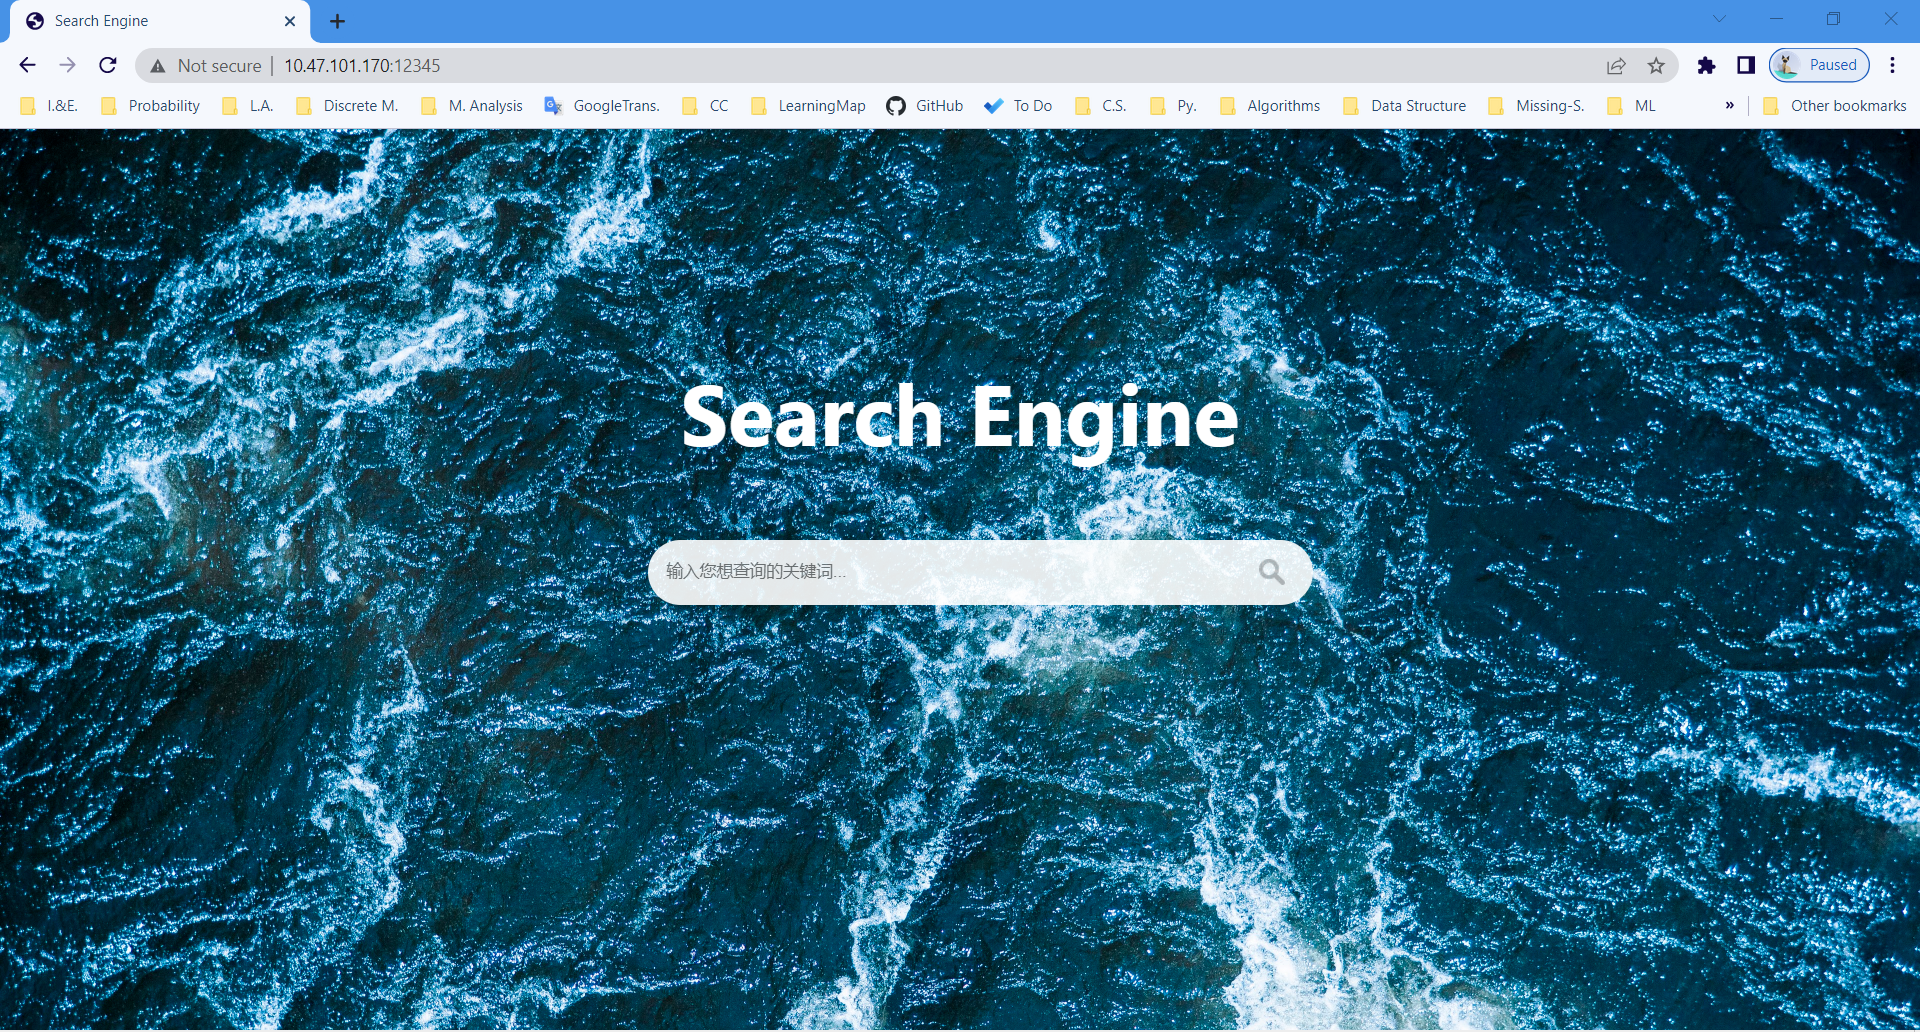
\includegraphics[
width=1\textwidth]{index_page}
\end{figure}
\begin{figure}[h]
\centering
\includegraphics[
width=1\textwidth]{result_page}
\end{figure}
\section{致谢}
衷心感谢中国人民大学高瓴人工智能学院毛佳昕老师的精彩授课与悉心指导,以及两位助教师兄的建议与帮助。
\end{document}
